\documentclass[a4paper,10pt]{article}

\usepackage[utf8]{inputenc}
\usepackage[T1]{fontenc}
\usepackage[english]{babel}

\usepackage{color}
\usepackage{float}
\usepackage{fancyvrb}

\usepackage{amssymb}
\usepackage{amsmath}

\usepackage{listings}
\usepackage{comment}
\usepackage[boxed]{algorithm2e}
\usepackage{graphicx}
\usepackage{subcaption}
\usepackage{subfig}

\usepackage{amsthm}
\theoremstyle{plain}

\theoremstyle{definition}
\newtheorem{defn}{Definition}
% \begin{defn}Here is a new definition.\end{defn}

\DeclareGraphicsExtensions{.png}

\definecolor{dkgreen}{rgb}{0,0.45,0}
\definecolor{gray}{rgb}{0.5,0.5,0.5}
\definecolor{mauve}{rgb}{0.30,0,0.30}

\lstset{frame=tb,
  language=Java,
  aboveskip=3mm,
  belowskip=3mm,
  showstringspaces=false,
  columns=flexible,
  basicstyle={\small\ttfamily},
  numbers=left,
  numberstyle=\footnotesize,
  keywordstyle=\color{dkgreen}\bfseries,
  commentstyle=\color{red},
  stringstyle=\color{mauve},
  frame=single,
  breaklines=true,
  breakatwhitespace=false
  tabsize=1
}

\title{ Parameterless clustering by dynamic tree-cutting \rule{10cm}{0.5mm}}
\author{Simon Lehmann Knudsen \\
	simkn15@student.sdu.dk \\
	ECTS: 10 \\
	04/09-2017 - 31/01-2018 \\
	5th semester in Computer Science
\\\rule{5.5cm}{0.5mm}\\}
\date{31/01-2018}

\begin{document}
\maketitle

\newpage
\tableofcontents

\begin{comment}
\begin{itemize}
	\item 1.4 What is a cluster? (Cluster Analysis)
	\item Description of clustering approaches: (Article) On Clustering validation technique
	\item Add description of clustering algorithms to appendix section
	\item Figure \ref{fig:hc example}: Needs to redo this, such that use "Cluster" and not "Partitioning".
	\item Describe unsupervised learning and supervised learning (Need to fine a proper place to put it)
	\item add Steps of clustering process to introduction (On Clustering Validation Techniques)
	\item References External/Internal at section background -> Cluster validation???
\end{itemize}
\end{comment}

%%%%%%%%%%%%%%%%%%%%%%%%%%%%%%%%%%%%%%%%%%%%%%%%%%
%%%%%%%%%%%%%%%%%%%%%%%%%%%%%%%%%%%%%%%%%%%%%%%%%%
%%%%%%%%%%%%%%%%%%%%%%%%%%%%%%%%%%%%%%%%%%%%%%%%%%
\newpage
\section{Abstract}
%%%%%%%%%%%%%%%%%%%%%%%%%%%%%%%%%%%%%%%%%%%%%%%%%%
%%%%%%%%%%%%%%%%%%%%%%%%%%%%%%%%%%%%%%%%%%%%%%%%%%
%%%%%%%%%%%%%%%%%%%%%%%%%%%%%%%%%%%%%%%%%%%%%%%%%%

%%%%%%%%%%%%%%%%%%%%%%%%%%%%%%%%%%%%%%%%%%%%%%%%%%
%%%%%%%%%%%%%%%%%%%%%%%%%%%%%%%%%%%%%%%%%%%%%%%%%%
\subsection{Background}
%%%%%%%%%%%%%%%%%%%%%%%%%%%%%%%%%%%%%%%%%%%%%%%%%%
%%%%%%%%%%%%%%%%%%%%%%%%%%%%%%%%%%%%%%%%%%%%%%%%%%

%%%%%%%%%%%%%%%%%%%%%%%%%%%%%%%%%%%%%%%%%%%%%%%%%%
%%%%%%%%%%%%%%%%%%%%%%%%%%%%%%%%%%%%%%%%%%%%%%%%%%
\subsection{Results}
%%%%%%%%%%%%%%%%%%%%%%%%%%%%%%%%%%%%%%%%%%%%%%%%%%
%%%%%%%%%%%%%%%%%%%%%%%%%%%%%%%%%%%%%%%%%%%%%%%%%%

%%%%%%%%%%%%%%%%%%%%%%%%%%%%%%%%%%%%%%%%%%%%%%%%%%
%%%%%%%%%%%%%%%%%%%%%%%%%%%%%%%%%%%%%%%%%%%%%%%%%%
\subsection{Conclusion}
%%%%%%%%%%%%%%%%%%%%%%%%%%%%%%%%%%%%%%%%%%%%%%%%%%
%%%%%%%%%%%%%%%%%%%%%%%%%%%%%%%%%%%%%%%%%%%%%%%%%%

%%%%%%%%%%%%%%%%%%%%%%%%%%%%%%%%%%%%%%%%%%%%%%%%%%
%%%%%%%%%%%%%%%%%%%%%%%%%%%%%%%%%%%%%%%%%%%%%%%%%%
%%%%%%%%%%%%%%%%%%%%%%%%%%%%%%%%%%%%%%%%%%%%%%%%%%
\newpage
\section{Introduction}
%%%%%%%%%%%%%%%%%%%%%%%%%%%%%%%%%%%%%%%%%%%%%%%%%%
%%%%%%%%%%%%%%%%%%%%%%%%%%%%%%%%%%%%%%%%%%%%%%%%%%
%%%%%%%%%%%%%%%%%%%%%%%%%%%%%%%%%%%%%%%%%%%%%%%%%%
% General clustering
% Clustering problem
% Inspiration from article 'Comprehensive cluster analysis with Transitivity Clustering'
% Could be interesting looking in Cluster Analysis
% Look at notes.tex

In ancient history it was important to realize that many objects shared certain properties like being edible or poisonous. Since it could be a matter of living or dieing. Categorizing is something most people, if not all, are doing daily without paying too much attention to it. Categorizing, or classifying, people as cute, clever, marriage-potential, etc..

Two key learnings methods are: (Does not fit here)
\begin{itemize}
	\item \textbf{Supervised Learning}: The machine learning task of inferring a function $f : X \rightarrow Y$ given a set of labeled training data $\{ \langle x_i, y_i \rangle \}$. 
	\item \textbf{Unsupervised Learning}: The task of building a model of X explaining its structure and inherit properties.
\end{itemize}
In short the difference is that supervised learning has a training data given a priori, where there is none in unsupervised learning. Thus, making supervised learning more subjective. Clustering is an unsupervised learning method.


%%%%%%%%%%%%%%%%%%%%%%%%%%%%%%%%%%%%%%%%%%%%%%%%%%
%%%%%%%%%%%%%%%%%%%%%%%%%%%%%%%%%%%%%%%%%%%%%%%%%%
\subsection{What is Clustering?}
%%%%%%%%%%%%%%%%%%%%%%%%%%%%%%%%%%%%%%%%%%%%%%%%%%
%%%%%%%%%%%%%%%%%%%%%%%%%%%%%%%%%%%%%%%%%%%%%%%%%%  
Clustering, or cluster analysis, is a way of grouping a set of objects such that a cluster (group) of objects is more similar to each other than those of another cluster. Clustering can help with the description of patterns of similarities and differences in a data set. Similarity is highly subjective depending on the scenario.
How a cluster is recognized is not entirely clear when displayed in the plane. One intuitive approach is assessing the relative distances between points. Figure \ref{fig:clusterShapes} shows three types of shapes for clusters. Looking at the middle one, assessing the distance between points would not necessarily give two clusters. Taking the left cluster, shape of the letter \textbf{C}. The top most right point and the bottom most right point would have a high distance insinuating low similarity. Visually the two points are in the same cluster. 
Figure \ref{fig:noNaturalCluster} shows an example without any 'natural' clusters. Visual examination does not leave any clues on the number of clusters. This scenario can be the geographical locations of houses in a town, where it makes sense to divide the houses into postal districts. Clustering is used in many different fields like market research, astronomy, weather classification, bioinformatics and genetics, etc..
\begin{figure}[H]
	\centering
	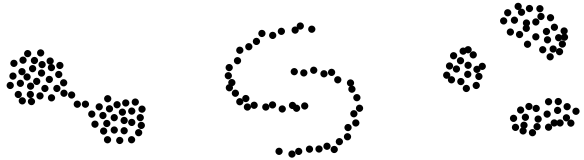
\includegraphics[scale=0.4]{./pictures/clusterShapes.png}
	\caption{Different shapes of clusters}
	\label{fig:clusterShapes}
\end{figure}
\begin{figure}[H]
	\centering
	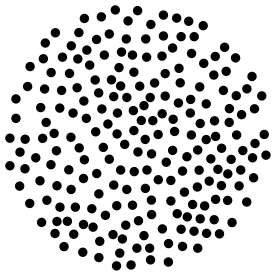
\includegraphics[scale=0.4]{./pictures/noNaturalCluster.png}
	\caption{}
	\label{fig:noNaturalCluster}
\end{figure}

There are many different tools to do cluster analysis, which all intend to find an optimal clustering depending on a set of criteria. Given a set of criteria and parameters, we can analyze the data and discover the clusters. The resulting clusters can all be either feasible or infeasible. In some circumstances overlapping clusters can provide acceptable solutions. When there are no clear separation of clusters, it can be hard to determine if the solution is acceptable or not.\\
Figure \ref{fig:g2-combined} shows similar datasets with decreasing separating and density of the clusters. \texttt{g2-2-70} does not have any clear separation between the clusters, and visually determining the number of clusters is no longer an option.
\begin{figure}[H]
	\centering
	\begin{minipage}{5cm}
		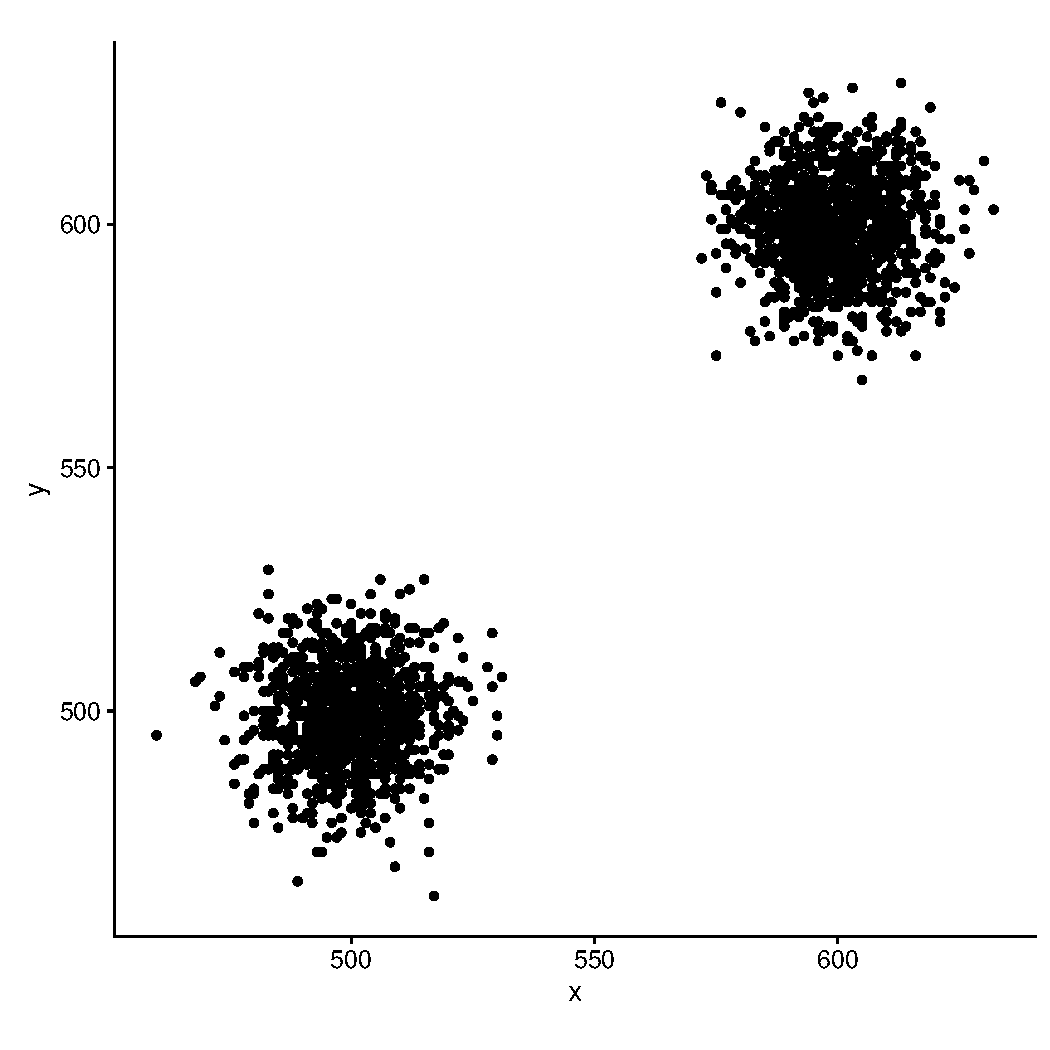
\includegraphics[width=5cm]{./pictures/G2/g2-2-10.pdf}
		\caption*{g2-2-10}
		\label{g2-2-10}
	\end{minipage}
	\begin{minipage}{5cm}
		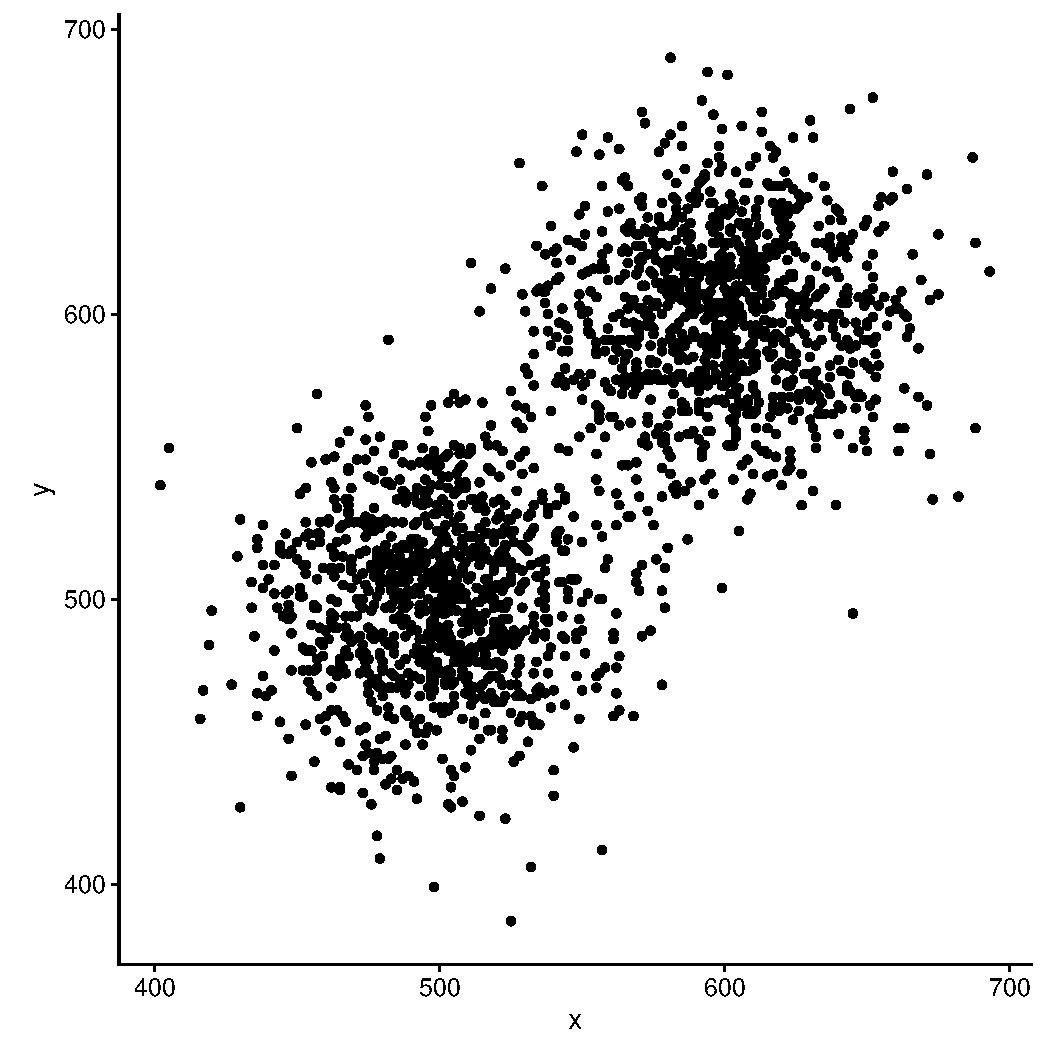
\includegraphics[width=5cm]{./pictures/G2/g2-2-30.pdf}
		\caption*{g2-2-30}
		\label{g2-2-30}
	\end{minipage}
	\\
	\begin{minipage}{5cm}
		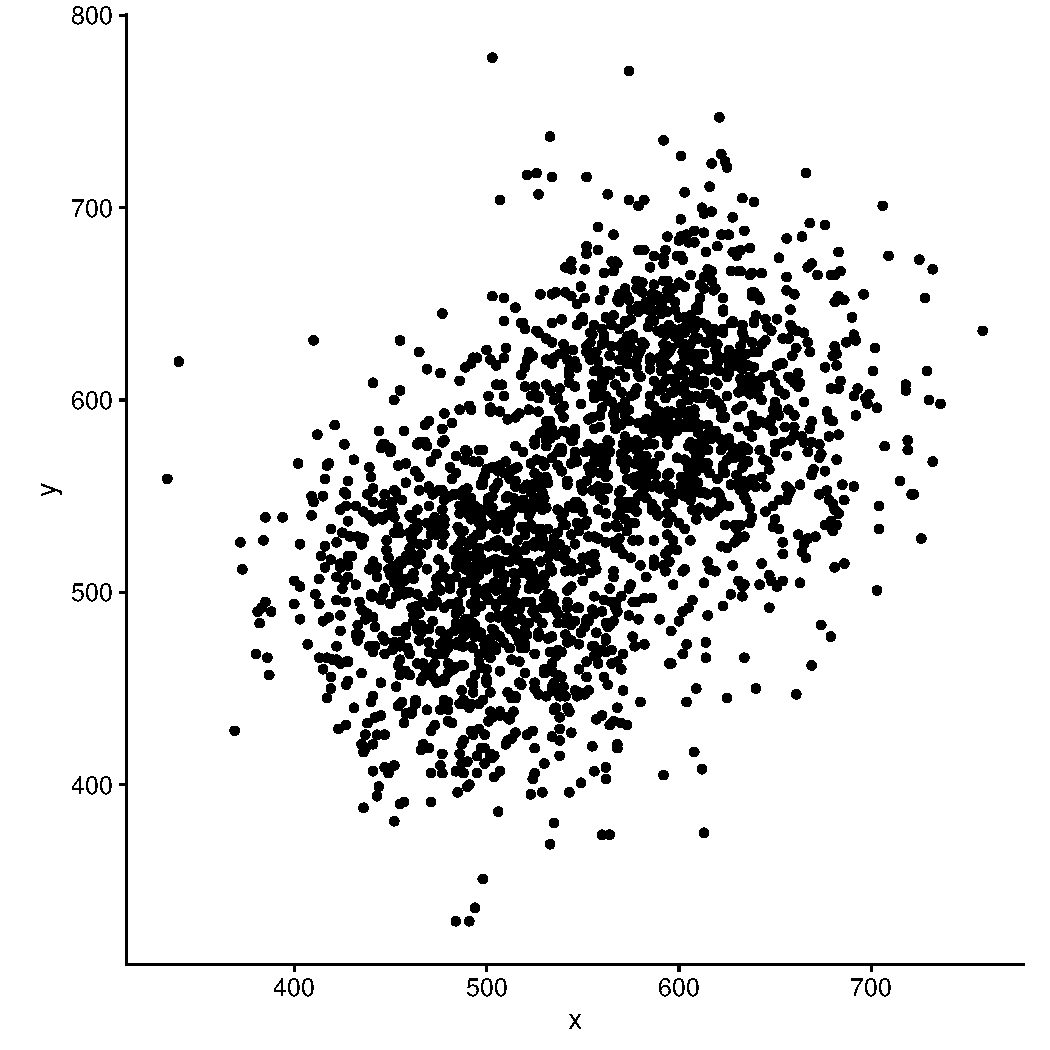
\includegraphics[width=5cm]{./pictures/G2/g2-2-50.pdf}
		\caption*{g2-2-50}
		\label{g2-2-50}
	\end{minipage}
	\begin{minipage}{5cm}
		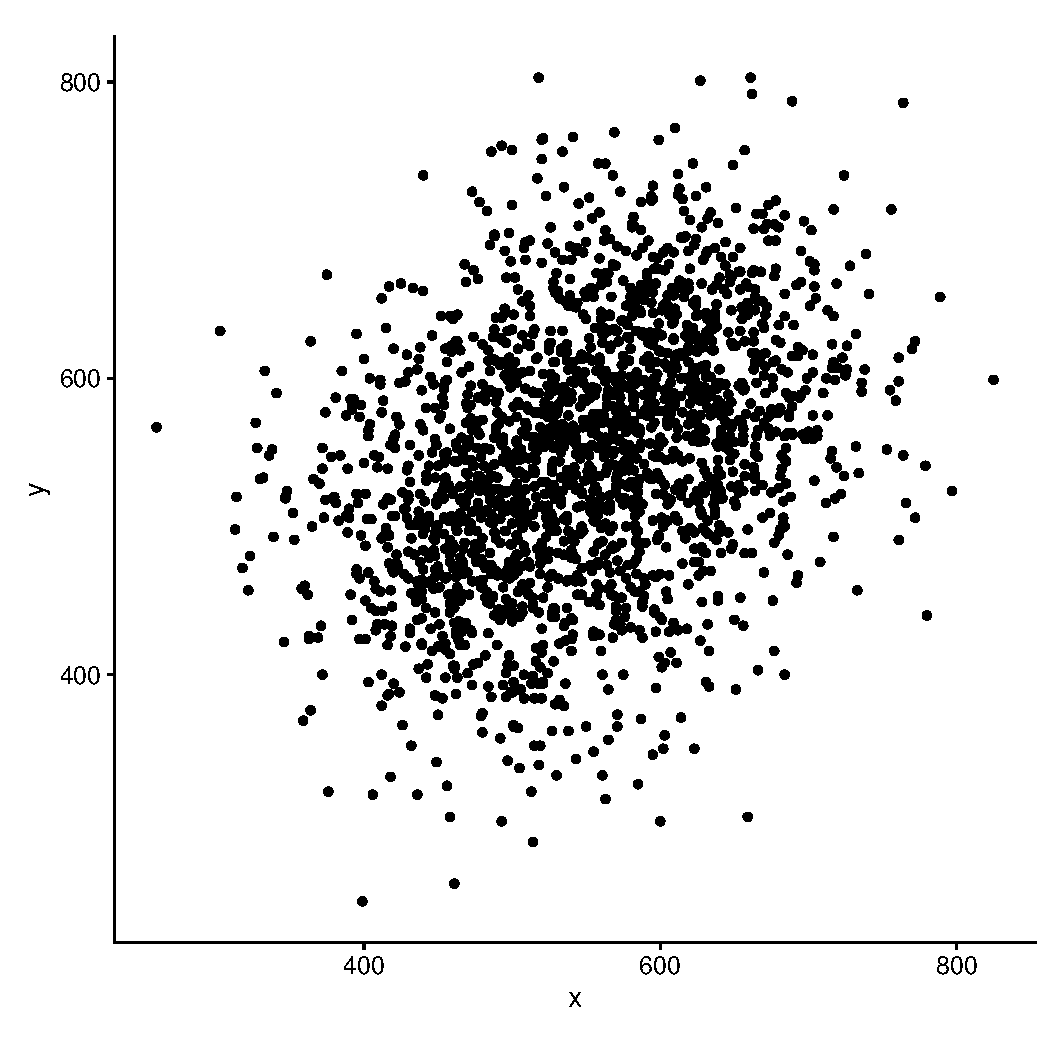
\includegraphics[width=5cm]{./pictures/G2/g2-2-70.pdf}
		\caption*{g2-2-70}
		\label{g2-2-70}
	\end{minipage}
	
	\caption{URL: https://cs.joensuu.fi/sipu/datasets/}
	\label{fig:g2-combined}
\end{figure}

\begin{figure}[H]
	\centering
	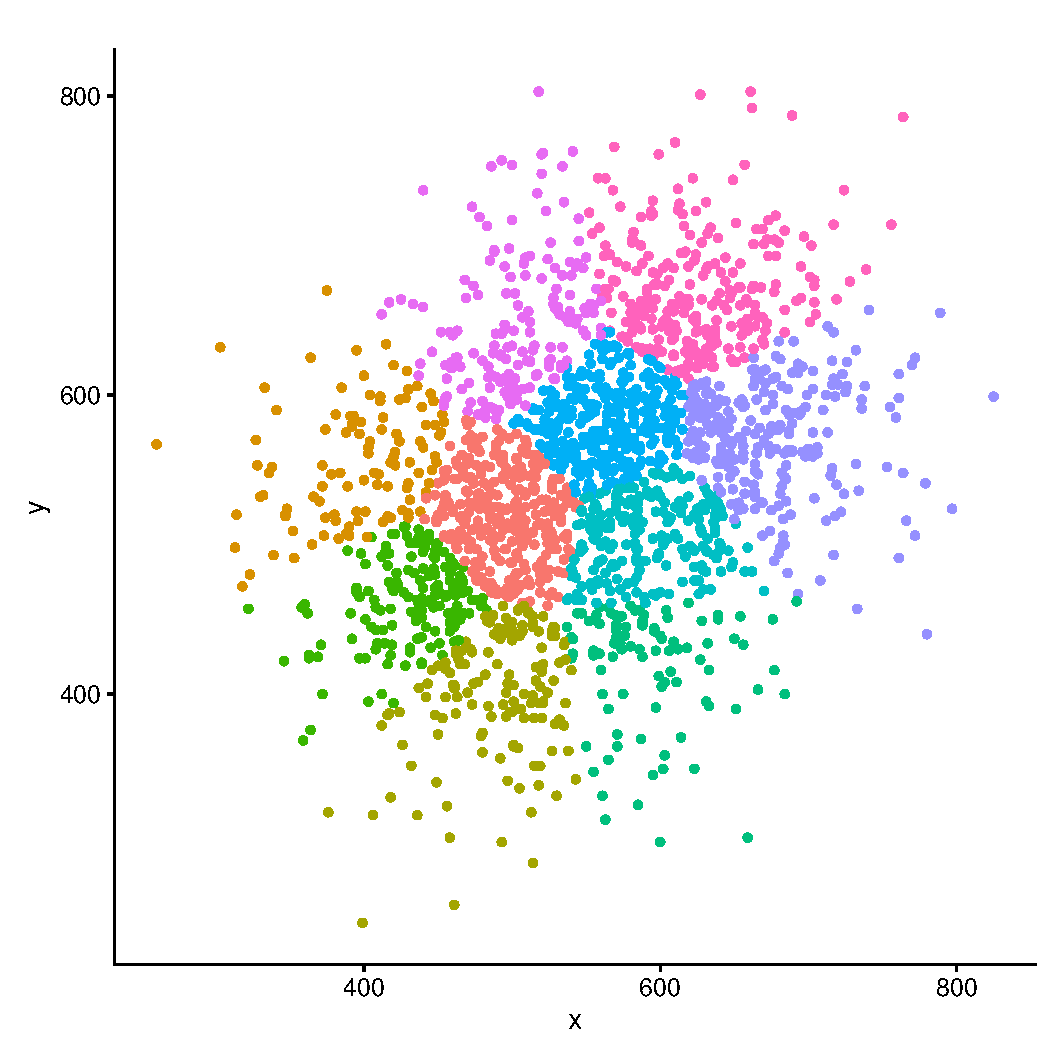
\includegraphics[scale=0.4]{./pictures/G2/g2-2-70-k10.pdf}
	\caption{g2-2-70 clustering with 10 clusters}
	\label{fig:g2-2-70-k10}
\end{figure}
Clustering requires an understanding of the dataset, in order to select the proper features of the data to determine the similarity. E.g. the optimal clustering solution could be one with 10 clusters, shown in figure \ref{fig:g2-2-70-k10}. A feature is some attribute which describes the data. Lets say the dataset was about the appearance of people. The features could be hair color, eye color, height, weight, etc..
The basic data for a cluster analysis starts with a $n \cdot p$ multivariate data matrix, \texttt{X}, which describes each object to be clustered. The entry $x_{ij}$ gives the value of the \textit{j}th variable on object \textit{i}:
\begin{figure}[H]
	\centering
	\[
	\texttt{X}
	=
	\begin{bmatrix}
	x_{11} & x_{12} & \dots & x_{1p} \\
	x_{21} & x_{22} & \dots & \dots \\
	\vdots & \vdots & \vdots & \vdots \\
	x_{n1} & \dots & \dots & x_{np}
	\end{bmatrix}
	\]
	\caption{Multivariate data matrix}
	\label{fig:dataMatrix}
\end{figure}

Many clustering techniques begins by converting \texttt{X} into a symmetric $n \cdot n$ matrix. Both rows and columns represents the objects in the data set. The resulting matrix could be of similarities, dissimilarities or distances between all objects.

%%%%%%%%%%%%%%%%%%%%%%%%%%%%%%%%%%%%%%%%%%%%%%%%%%
%%%%%%%%%%%%%%%%%%%%%%%%%%%%%%%%%%%%%%%%%%%%%%%%%%
\subsection{Clustering Approaches}
%%%%%%%%%%%%%%%%%%%%%%%%%%%%%%%%%%%%%%%%%%%%%%%%%%
%%%%%%%%%%%%%%%%%%%%%%%%%%%%%%%%%%%%%%%%%%%%%%%%%%
There are many different clustering approaches. Each has its purpose dependent on the data. The three most notable approaches are
\begin{itemize}
	\item \textbf{Partitional}: Requires a parameter k, which is the number of returned clusters while optimizing a criterion function, e.g. a distance function.
	\item \textbf{Hierarchical}: Proceeds by either merging smaller clusters into larger, or splitting larges cluster into smaller. Resulting in a dendrogram, which is a tree of clusters, showing the related clusters. The clustering solution is given by a cut on a desired level of the dendrogram.
	\item \textbf{Density-based}: Grouping neighboring objects into clusters based on a density condition.
\end{itemize}
With partitional clustering it can be hard to derive a proper k for the returned clusters. With low dimensional data plotting the data can be helpful to determine k, but gets increasingly difficult with high dimensional data. As a rule of thumb $1 \ll k \leq 10$. Calculating the F-ratio can possible give a good estimation for k.
Density-based clustering is usually not a good approach if the dataset has a high variance of density between the clusters.
Next is some algorithms under each approach
%%%%%%%%%%%%%%%%%%%%%%%%%%%%%%%%%%%%%%%%%%%%%%%%%%
%%%%%%%%%%%%%%%%%%%%%%%%%%%%%%%%%%%%%%%%%%%%%%%%%%
\begin{itemize}
	\item \textbf{Reference: On Clustering Validation Techniques}
	\item Partitional algorithms
	\subitem K-Means
	\subitem PAM (Partitioning Around Medoids)
	\subitem CLARA (Clustering Large Applications)
	\subitem CLARANS (Clustering Large Applications based on Randomized Search)
	\item Hierarchical algorithms:
	\subitem Agglomerative algorithms:
	\subitem Divisive algorithms:
	\subitem BIRCH (Zhang et al., 1996)
	\subitem CURE (Guha et al., 1998)
	\subitem ROCK (Guha et al., 1999)
	\item Density-based algorithms
	\subitem DBSCAN
	\subitem DENCLUE
	\subitem Transitivity Clustering (TC)
	
	A description of the algorithms can be found in the appendix section(Missing at the moment)
\end{itemize}
For this project the density-based algorithm Transitivity Clustering is used, and is incorporated into a hierarchical clustering approach.

%%%%%%%%%%%%%%%%%%%%%%%%%%%%%%%%%%%%%%%%%%%%%%%%%%
%%%%%%%%%%%%%%%%%%%%%%%%%%%%%%%%%%%%%%%%%%%%%%%%%%
\subsection{Cluster validity}
%%%%%%%%%%%%%%%%%%%%%%%%%%%%%%%%%%%%%%%%%%%%%%%%%%
%%%%%%%%%%%%%%%%%%%%%%%%%%%%%%%%%%%%%%%%%%%%%%%%%%
It is difficult to visually compare two clusterings if they differ in a few points, thus it is needed to calculate the quality of a clustering. Clustering is a unsupervised learning where are no training data to guide, so how do we measure the quality? There are many different methods, and which one to use can be different depending on the data.
To validate a clustering there are two methods, internal measures and external measures. Internal measures are often based on
\begin{itemize}
	\item Compactness: Measures how closely related the objects are in a cluster
	\item Separation: Measures how distinct or well-separated a cluster is from other clusters
\end{itemize}
Internal measures are e.g. Sum of Squares(SSQ), Silhouette Coefficient and Dunn Index. External measures use external information not present in the data. Normally a 'gold standard' is used. A gold standard is a clustering solution developed by experts, and are rarely available. Comparing against this ground truth is the way for determining the quality. External measures are e.g. F-measure and Jaccard coefficient. For this project F-measure is the used quality measure and will be further discussed later.


%%%%%%%%%%%%%%%%%%%%%%%%%%%%%%%%%%%%%%%%%%%%%%%%%%
%%%%%%%%%%%%%%%%%%%%%%%%%%%%%%%%%%%%%%%%%%%%%%%%%%
%%%%%%%%%%%%%%%%%%%%%%%%%%%%%%%%%%%%%%%%%%%%%%%%%%
\newpage
\section{Background}
%%%%%%%%%%%%%%%%%%%%%%%%%%%%%%%%%%%%%%%%%%%%%%%%%%
%%%%%%%%%%%%%%%%%%%%%%%%%%%%%%%%%%%%%%%%%%%%%%%%%%
%%%%%%%%%%%%%%%%%%%%%%%%%%%%%%%%%%%%%%%%%%%%%%%%%%

%%%%%%%%%%%%%%%%%%%%%%%%%%%%%%%%%%%%%%%%%%%%%%%%%%
%%%%%%%%%%%%%%%%%%%%%%%%%%%%%%%%%%%%%%%%%%%%%%%%%%
\subsection{The Dataset}
%%%%%%%%%%%%%%%%%%%%%%%%%%%%%%%%%%%%%%%%%%%%%%%%%%
%%%%%%%%%%%%%%%%%%%%%%%%%%%%%%%%%%%%%%%%%%%%%%%%%%
% Inspiration for description of brown: 'Partitional biological data with transitivity clustering' "A typical clustering workflow by using a gold standard data set of enzyme families"
% Reference?: S. D. Brown, J. A. Gerlt, J. L. Seffernick et al., Genome Biol 7 (1), R8 (2006).

%%%%%%%%%%%%%%%%%%%%%%%%%%%%%%%%%%%%%%%%%%%%%%%%%%
%%%%%%%%%%%%%%%%%%%%%%%%%%%%%%%%%%%%%%%%%%%%%%%%%%
\subsection{Transitivity Clustering}
%%%%%%%%%%%%%%%%%%%%%%%%%%%%%%%%%%%%%%%%%%%%%%%%%%
%%%%%%%%%%%%%%%%%%%%%%%%%%%%%%%%%%%%%%%%%%%%%%%%%%
% article 'Comprehensive cluster analysis with Transitivity Clustering'
% article 'Partitioning biological data with transitivity clustering'
% article 'Large scale clustering of protein sequence with FORCE-A layout based heuristic for weighted cluster editing'

Before going into any details about Transitivity Clustering(TC) we need some basic graph-theoretic definitions.
\begin{description}
	\item[Definitions from 'Extension and Robustness of Transitivity Clustering for Protein...']
\end{description}

\begin{defn}[\texttt{Undirected simple graph}]\label{def:Undirected simple graph}
	An \texttt{undirected simple graph} $G = (V, E)$ consists of a set of nodes V and a set of edges $E \subseteq {V \choose 2}$, where ${V \choose 2}$ denotes the set of two-element subsets of V. The edges are undirected and contains no self-loops or multiple edges between two nodes. \textit{uv} is an unordered par $\{u, v \} \in {V \choose 2}$.
\end{defn}

\begin{defn}[\texttt{Transitive graph}]\label{def:Transitive graph}
	An undirected simple graph $G = (V, E)$ is called \texttt{transitive} 
	\begin{equation*}
	\text{if for all triples } uvw \in {V \choose 3}, uv \in E \text{ and } vw \in E \text{ implies } uw \in E.
	\end{equation*}
\end{defn}

\begin{defn}[\texttt{Weighted Transitive Graph Projection Problem(WTGPP)}]\label{def:WTGPP}
	 Given a set of objects \texttt{V}, a threshold $t \in \mathbb{R}$, and a pairwise similarity function sim: ${V \choose 2} \rightarrow \mathbb{R}$, the graph \textit{G} is defined as
	 \begin{equation}\label{eq:sim above threshold}
	 G = (V, E); \; E = \bigg\{ uv \in {V \choose 2} : \text{sim}(uv) > t\bigg\}
	 \end{equation}
	 The WTGPP is the determination of a transitive graph $G' = (V, E')$ such that there exist no other transitive graph $G'' = (V, E'')$ with $\text{cost}(G \rightarrow G'') < \text{cost}(G \rightarrow G')$. The modification costs are defined as
	 \begin{equation}\label{eq:TC cost function}
		 \text{cost}(G \rightarrow G') := \underbrace{\sum_{uv \in E \backslash E'} | \text{sim}(uv) - t |}_{\text{deletion cost}} + \underbrace{\sum_{uv \in E' \backslash E} | \text{sim}(uv) - t |}_{\text{addition cost}}
	 \end{equation}
\end{defn}

% Briefly write about the steps in the "algorithm" from article 'Comprehensive cluster analysis with trans clust'
% Talk about R package ????? (implementation section ?)

Transitivity Clustering takes one parameter, \textit{t}, which is the threshold for similarities. Following is the steps in Transitivity Clustering: \\
\textbf{Reference: Comprehensive cluster analysis with Transitivity Clustering}
\begin{enumerate}
	\item Model the given pairwise similarity, from the similarity matrix, as a similarity graph, \textit{G}. The nodes corresponds to the objects, with weighted edges as the similarity values.
	
	\item Transform the similarity graph, \textit{G}, into another graph, \textit{G'}, by subtracting the threshold from the edge weights. Subsequently removing those edges with weights below zero, which is the deletion cost for equation \ref{eq:TC cost function}.
	
	\item Transform \textit{G'} into a transitive graph, \textit{G''}, with minimal cost. Thus, in this step we add all edges such that the graph is transitive, which is the addition cost for equation \ref{eq:TC cost function}.
\end{enumerate}
The resulting transitive graph, \textit{G''}, is the clustering solution.


%%%%%%%%%%%%%%%%%%%%%%%%%%%%%%%%%%%%%%%%%%%%%%%%%%
%%%%%%%%%%%%%%%%%%%%%%%%%%%%%%%%%%%%%%%%%%%%%%%%%%
\subsection{Hierarchical Clustering}
%%%%%%%%%%%%%%%%%%%%%%%%%%%%%%%%%%%%%%%%%%%%%%%%%%
%%%%%%%%%%%%%%%%%%%%%%%%%%%%%%%%%%%%%%%%%%%%%%%%%%
% Chapter 4 from Cluster Analysis book
% Cluster Analysis: Look at Agglomerative(4.2) and Divisive (4.3)
% Look at notes.tex

\begin{defn}[\texttt{Hierarchical Clustering(HC)}]\label{def:hc}
	\textbf{Reference from Unsupervised Learning slides: Hierarchical Clustering}\\
	Builds a nested structural partition $C = 	\{ C_1, \dots, C_k\}$ of \textit{V} such that $\cup_{i = 1}^{k} C_i = V$ and $C_i \neq \emptyset$ $\forall i \in \{1, \dots, k\}$. $\forall \text{ pairs } C_i, C_j$ where $i,j \in \{1, \dots, k\}, i \neq j$, exactly one of the following holds
	\begin{itemize}
		\item $C_i \cap C_j = \emptyset$
		\item $C_i \subset C_j$
		\item $C_j \subset C_i$
	\end{itemize}
\end{defn}

There are two forms of hierarchical Clustering, \texttt{agglomerative} and \texttt{divisive}. Agglomerate starts with \textit{n} clusters, where \textit{n} is the number of objects in the data set. Joining clusters until one cluster is remaining, where all \textit{n} objects are members. Divisive is the opposite. Starting with one cluster with \textit{n} objects. Splitting the clusters until all clusters are singletons. Thus, all \textit{n} objects represents are cluster. Agglomerative is the most used, as divisive usually is a more expensive procedure. One important feature of hierarchical clustering is that a join or split of clusters are irrevocable, thus cannot be undone. Figure \ref{fig:agglo_vs_div} shows an overview of agglomerative vs. divisive.
\begin{figure}[H]
	\centering
	\includegraphics*[scale=0.3]{./pictures/hc/agglo_vs_div.png}
	\caption{Agglomerative vs. Divisive: Reference Cluster Analysis, page 72}
	\label{fig:agglo_vs_div}
\end{figure} 
The steps of joins or splits is often showed as a \texttt{dendrogram}, which is viewed as a tree structure. The root of the tree is the cluster containing all \textit{n} objects. Moving down the tree the nodes represents the clusters which was split from its parent. At the bottom of the tree we have the leafs, where the number of leafs represents all singleton clusters(the \textit{n} objects). The tree can be cut a given height resulting in a clustering solution. Figure \ref{fig:hc example} shows a \texttt{dendrogram} of the tree structure of a HC. The horizontal axis shows all the objects in the data set. The vertical axis shows the distances between objects and/or clusters. Objects 1 and 2 are joined to a cluster at height 2. These are joined with the remaining objects at height 5, resulting in one cluster holding all objects.
\begin{figure}[H]
	\centering
	\includegraphics*[scale=0.3]{./pictures/hc/hc_example.png}
	\caption{Dendrogram of a Hierarchical Clustering: Reference Cluster Analysis, page 75}
	\label{fig:hc example}
\end{figure}

In a typical hierarchical Clustering the size and number of clusters are given by a threshold, much like the one used in \texttt{TC}. Meaning that one iteration can possibly affect all clusters, which either increases or decreases the overall quality. In Figure \ref{fig:hc example} the tree could be cut between distance 3-4 to obtain a solution containing three clusters.
\begin{comment}
\\\textbf{Not the right section explaining about cutting the tree to gain optimal solution(Dynamic tree cut)}\\
In Figure \ref{fig:hc quality example} we could cut the tree between height 3-7.5 and we would get a solution containing two clusters. One issue in terms of quality is that, the optimal clustering solution could have the clusters {5, 2}, {3, 6, 1},  {7} and {4, 0}. Making a horizontal cut in the tree, it would be impossible to obtain this solution. However, if it was possible to make a dynamic tree cut, the optimal solution could in fact be obtained. The solution can be made by cutting the tree in three different heights. First cut is between 2.5 and 7.5 to obtain the cluster {5, 1}. Cutting between height 2.0 and 3.0, obtaining cluster {3, 6, 1}. The last cut is between 2.5 and 3, giving the last clusters {7} and {4, 0}.
\begin{figure}[H]
	\centering
	\includegraphics*[scale=0.4]{./pictures/hc/hc_quality_example.png}
	\caption{Reference: Slides Hierarchical Clustering}
	\label{fig:hc quality example}
\end{figure}
\end{comment}


%%%%%%%%%%%%%%%%%%%%%%%%%%%%%%%%%%%%%%%%%%%%%%%%%%
%%%%%%%%%%%%%%%%%%%%%%%%%%%%%%%%%%%%%%%%%%%%%%%%%%
\subsection{Cluster Validation - F-measure}
%%%%%%%%%%%%%%%%%%%%%%%%%%%%%%%%%%%%%%%%%%%%%%%%%%
%%%%%%%%%%%%%%%%%%%%%%%%%%%%%%%%%%%%%%%%%%%%%%%%%%
% Section 'Partitioning biological data with Transitivity Clustering'
% Look at source.tex in articles folder
Often it is crucial to measure the quality of a clustering result. Evaluating the best of two results can be difficult, if not impossible, when looking at plots of the clusterings. Thus, we need other methods to validate the results. \texttt{Cluster validity indexes} are a important factor to evaluate solutions. There are three categories of cluster validity indexes:
\begin{itemize}
	\item External Criteria/Validation: Evaluate the result with respect to a pre-specified structure, such as a gold standard. 
	\item Internal Criteria/Validation: Evaluate the result with respect to information intrinsic to the data alone.
	\item Relative Criteria: Choosing the best clustering scheme of a set of defined schemes, according to a pre-specified criterion.
\end{itemize}
We are using the brown data set, which has a gold standard. Thus, we can evaluate results with the external criteria. F-measure falls under this category, and is the chosen quality measure.There are multiple versions of the F-measure. We will be using the $\text{F}_1-measure$, where the measures Recall and Precision is weighted equally. In order to understand the F-measure we need the following definitions:\\
$K = (K_1, \dots, K_m) = $ Clustering result obtained from the algorithm. $K_i$ is the \textit{i}th cluster in \textit{K}.\\
$G = (G_1, \dots, G_l) = $ Gold standard clustering. $G_j$ is the \textit{j}th cluster in \textit{G}.\\
$n = $ amount of objects in the data set. \\
$n_i = $ number of objects in cluster $K_i$. \\
$n^j = $ number of objects in cluster $C_j$. \\
$n_{i}^{j} = $ number of objects contained in $K_i \cap C_j$

\begin{defn}[True Positive]\label{}
	The number of common objects between cluster \textit{i} and the compared gold standard cluster \textit{j}.
	\begin{equation}
		\text{TP} = |K_i \cup C_j|
	\end{equation}
\end{defn}

\begin{defn}[False Positive]\label{}
	The number of objects in cluster \textit{i}, which are not in the compared gold standard cluster \textit{j}.
	\begin{equation}
		\text{FP} = |K_i \backslash C_j|
	\end{equation}
\end{defn}

\begin{defn}[False Negative]\label{}
	The number of objects that are not in cluster \textit{i}, which are in the compared gold standard cluster \textit{j}
	\begin{equation}
		\text{FN} = |C_j \backslash K_i|
	\end{equation}
\end{defn}

\begin{defn}[Recall]\label{}
	\begin{equation}
		\text{Recall}(i,j) = \frac{n_{ij}}{n_i} = \frac{TP}{TP + FP}
	\end{equation}
\end{defn}

\begin{defn}[Precision]\label{}
	\begin{equation}
		\text{Precision}(i,j) = \frac{n_{ij}}{n_j} = \frac{TP}{TP + FN}
	\end{equation}
\end{defn}

\begin{defn}[F-measure for a cluster]\label{}
	The F-measure of cluster \textit{j} and class \textit{i} is given by:
	\begin{equation}
		F(i,j) = 2 \cdot \frac{\text{Recall}(i,j) \cdot \text{Precision}(i,j)}{\text{Precision}(i,j) + \text{Recall}(i,j)}
	\end{equation}
\end{defn}

\begin{defn}[F-Measure for a clustering]\label{def:mean F-measure}
	In order to obtain the F-measure for a clustering solution, we need to find the mean F-measure. The F-measure of a cluster \textit{j} is multiplied by the amount of objects in the gold standard cluster which have most in common objects. Take the sum over all clusters. Divide by total amount of objects in the data set. Each cluster from the gold standard can only be referenced/mapped once.
	\begin{equation}
		\frac{\sum_{i = 1}^{m} \text{F-measure}(K_i) \cdot n_{i}^{j}}{n}
	\end{equation}
\end{defn}
A F-measure is between 0 and 1. A value near 1 indicates a good match with the gold standard(good clustering result). Values near 0 indicates a bad result. It is important to pay attention to the statement in Definition \ref{def:mean F-measure} saying that each cluster from the gold standard can only be referenced once. If, e.g. three clusters from \textit{K} maps to the same cluster in \textit{C}, two clusters will be neglected. The F-measure will be 0.0 for the neglected clusters, which negatively influences the quality. This scenario can happen in all clustering solutions, but the probability for multiple mappings on to the same gold standard cluster increases when $|K|>|C|$. In the opposite direction the scenario where $|K|<|C|$, also has a negative impact. With $|K|<|C|$ the clusters in K would be bigger than the cluster in C. 
Looking back at Definition \ref{def:mean F-measure}, we see that the multiplication is done with the size of $C_j$. Therefore we can conclude that the amount of objects that $K_i$ is bigger than $C_j$, $|K_i|-|C_j|$, has a smaller influence on the total F-measure than the remaining objects in $K_i$.


%%%%%%%%%%%%%%%%%%%%%%%%%%%%%%%%%%%%%%%%%%%%%%%%%%
%%%%%%%%%%%%%%%%%%%%%%%%%%%%%%%%%%%%%%%%%%%%%%%%%%
\subsection{Multidimensional Scaling}
%%%%%%%%%%%%%%%%%%%%%%%%%%%%%%%%%%%%%%%%%%%%%%%%%%
%%%%%%%%%%%%%%%%%%%%%%%%%%%%%%%%%%%%%%%%%%%%%%%%%%
\begin{comment}
Look at section 2.3.3 Multidimensional scaling (Cluster Analysis)

High dimensionality -> Curse of dimensionality (From slides)
Dimensionality reduction(From slides)


The issue when randomizing and low dimensionality. Hard if not impossible to have proper scale of similarities between many objects. If x1 and x2 have low similarity, but x3 have high similarity with both, which is higher than the middle between x1 and x2.
\end{comment}


%%%%%%%%%%%%%%%%%%%%%%%%%%%%%%%%%%%%%%%%%%%%%%%%%%
%%%%%%%%%%%%%%%%%%%%%%%%%%%%%%%%%%%%%%%%%%%%%%%%%%
\subsection{GAP Statistics}
%%%%%%%%%%%%%%%%%%%%%%%%%%%%%%%%%%%%%%%%%%%%%%%%%%
%%%%%%%%%%%%%%%%%%%%%%%%%%%%%%%%%%%%%%%%%%%%%%%%%%
% This is what is used for the reasoning of the randomization

%%%%%%%%%%%%%%%%%%%%%%%%%%%%%%%%%%%%%%%%%%%%%%%%%%
%%%%%%%%%%%%%%%%%%%%%%%%%%%%%%%%%%%%%%%%%%%%%%%%%%
%%%%%%%%%%%%%%%%%%%%%%%%%%%%%%%%%%%%%%%%%%%%%%%%%%
\newpage
\section{Method}
%%%%%%%%%%%%%%%%%%%%%%%%%%%%%%%%%%%%%%%%%%%%%%%%%%
%%%%%%%%%%%%%%%%%%%%%%%%%%%%%%%%%%%%%%%%%%%%%%%%%%
%%%%%%%%%%%%%%%%%%%%%%%%%%%%%%%%%%%%%%%%%%%%%%%%%%

%%%%%%%%%%%%%%%%%%%%%%%%%%%%%%%%%%%%%%%%%%%%%%%%%%
%%%%%%%%%%%%%%%%%%%%%%%%%%%%%%%%%%%%%%%%%%%%%%%%%%
\subsection{Assessing best clustering}
%%%%%%%%%%%%%%%%%%%%%%%%%%%%%%%%%%%%%%%%%%%%%%%%%%
%%%%%%%%%%%%%%%%%%%%%%%%%%%%%%%%%%%%%%%%%%%%%%%%%%
% This might be too similar with the sections under introduction ?

%%%%%%%%%%%%%%%%%%%%%%%%%%%%%%%%%%%%%%%%%%%%%%%%%%
%%%%%%%%%%%%%%%%%%%%%%%%%%%%%%%%%%%%%%%%%%%%%%%%%%
\begin{comment}
Skip writing about the failed approaches ?
Just stick to the one we are actually using ?
Richard mentioned we should describe the failed approaches, to reason about the one we are using.
(Look comment under "Results for randomizations")
\end{comment}
\subsection{Randomization approach 1}
%%%%%%%%%%%%%%%%%%%%%%%%%%%%%%%%%%%%%%%%%%%%%%%%%%
%%%%%%%%%%%%%%%%%%%%%%%%%%%%%%%%%%%%%%%%%%%%%%%%%%
% Look at notes.tex

%%%%%%%%%%%%%%%%%%%%%%%%%%%%%%%%%%%%%%%%%%%%%%%%%%
%%%%%%%%%%%%%%%%%%%%%%%%%%%%%%%%%%%%%%%%%%%%%%%%%%
\subsection{Randomization approach 2}
%%%%%%%%%%%%%%%%%%%%%%%%%%%%%%%%%%%%%%%%%%%%%%%%%%
%%%%%%%%%%%%%%%%%%%%%%%%%%%%%%%%%%%%%%%%%%%%%%%%%%
% Look at notes.tex

%%%%%%%%%%%%%%%%%%%%%%%%%%%%%%%%%%%%%%%%%%%%%%%%%%
%%%%%%%%%%%%%%%%%%%%%%%%%%%%%%%%%%%%%%%%%%%%%%%%%%
\subsection{Randomization approach 3}
%%%%%%%%%%%%%%%%%%%%%%%%%%%%%%%%%%%%%%%%%%%%%%%%%%
%%%%%%%%%%%%%%%%%%%%%%%%%%%%%%%%%%%%%%%%%%%%%%%%%%

%%%%%%%%%%%%%%%%%%%%%%%%%%%%%%%%%%%%%%%%%%%%%%%%%%
%%%%%%%%%%%%%%%%%%%%%%%%%%%%%%%%%%%%%%%%%%%%%%%%%%
\subsection{Randomization approach 4}
%%%%%%%%%%%%%%%%%%%%%%%%%%%%%%%%%%%%%%%%%%%%%%%%%%
%%%%%%%%%%%%%%%%%%%%%%%%%%%%%%%%%%%%%%%%%%%%%%%%%%

%%%%%%%%%%%%%%%%%%%%%%%%%%%%%%%%%%%%%%%%%%%%%%%%%%
%%%%%%%%%%%%%%%%%%%%%%%%%%%%%%%%%%%%%%%%%%%%%%%%%%
\subsection{Results for randomizations}
%%%%%%%%%%%%%%%%%%%%%%%%%%%%%%%%%%%%%%%%%%%%%%%%%%
%%%%%%%%%%%%%%%%%%%%%%%%%%%%%%%%%%%%%%%%%%%%%%%%%%
% Write about the results from the randomizations, and reasons to try other approaches.

%%%%%%%%%%%%%%%%%%%%%%%%%%%%%%%%%%%%%%%%%%%%%%%%%%
%%%%%%%%%%%%%%%%%%%%%%%%%%%%%%%%%%%%%%%%%%%%%%%%%%
%%%%%%%%%%%%%%%%%%%%%%%%%%%%%%%%%%%%%%%%%%%%%%%%%%
\newpage
\section{Implementation : Keep it short!}
%%%%%%%%%%%%%%%%%%%%%%%%%%%%%%%%%%%%%%%%%%%%%%%%%%
%%%%%%%%%%%%%%%%%%%%%%%%%%%%%%%%%%%%%%%%%%%%%%%%%%
%%%%%%%%%%%%%%%%%%%%%%%%%%%%%%%%%%%%%%%%%%%%%%%%%%

%%%%%%%%%%%%%%%%%%%%%%%%%%%%%%%%%%%%%%%%%%%%%%%%%%
%%%%%%%%%%%%%%%%%%%%%%%%%%%%%%%%%%%%%%%%%%%%%%%%%%
%%%%%%%%%%%%%%%%%%%%%%%%%%%%%%%%%%%%%%%%%%%%%%%%%%
\newpage
\section{Conclusion}
%%%%%%%%%%%%%%%%%%%%%%%%%%%%%%%%%%%%%%%%%%%%%%%%%%
%%%%%%%%%%%%%%%%%%%%%%%%%%%%%%%%%%%%%%%%%%%%%%%%%%
%%%%%%%%%%%%%%%%%%%%%%%%%%%%%%%%%%%%%%%%%%%%%%%%%%

%%%%%%%%%%%%%%%%%%%%%%%%%%%%%%%%%%%%%%%%%%%%%%%%%%
%%%%%%%%%%%%%%%%%%%%%%%%%%%%%%%%%%%%%%%%%%%%%%%%%%
%%%%%%%%%%%%%%%%%%%%%%%%%%%%%%%%%%%%%%%%%%%%%%%%%%
\newpage
\section{Appendix}
%%%%%%%%%%%%%%%%%%%%%%%%%%%%%%%%%%%%%%%%%%%%%%%%%%
%%%%%%%%%%%%%%%%%%%%%%%%%%%%%%%%%%%%%%%%%%%%%%%%%%
%%%%%%%%%%%%%%%%%%%%%%%%%%%%%%%%%%%%%%%%%%%%%%%%%%

%%%%%%%%%%%%%%%%%%%%%%%%%%%%%%%%%%%%%%%%%%%%%%%%%%
%%%%%%%%%%%%%%%%%%%%%%%%%%%%%%%%%%%%%%%%%%%%%%%%%%
\subsection{Clustering Approaches and Algorithms : Missing description of each algorithm}
%%%%%%%%%%%%%%%%%%%%%%%%%%%%%%%%%%%%%%%%%%%%%%%%%%
%%%%%%%%%%%%%%%%%%%%%%%%%%%%%%%%%%%%%%%%%%%%%%%%%%
\begin{itemize}
	\item \textbf{Reference: On Clustering Validation Techniques}
	\item Partitional algorithms
		\subitem K-Means
		\subitem PAM (Partitioning Around Medoids)
		\subitem CLARA (Clustering Large Applications)
		\subitem CLARANS (Clustering Large Applications based on Randomized Search)
	\item Hierarchical algorithms:
		\subitem Agglomerative algorithms:
		\subitem Divisive algorithms:
		\subitem BIRCH (Zhang et al., 1996)
		\subitem CURE (Guha et al., 1998)
		\subitem ROCK (Guha et al., 1999)
	\item Density-based algorithms
		\subitem DBSCAN
		\subitem DENCLUE
		\subitem Transitivity Clustering
	\item Grid-based algorithms
		\subitem STING (Statistical Information Grid-based method)
		\subitem WaveCluster
	\item Fuzzy clustering
		\subitem Fuzzy C-Means (FCM)
		\subitem EM (Expectation Maximization)
\end{itemize}

%%%%%%%%%%%%%%%%%%%%%%%%%%%%%%%%%%%%%%%%%%%%%%%%%%
%%%%%%%%%%%%%%%%%%%%%%%%%%%%%%%%%%%%%%%%%%%%%%%%%%
%%%%%%%%%%%%%%%%%%%%%%%%%%%%%%%%%%%%%%%%%%%%%%%%%%
\newpage
\section{References}
%%%%%%%%%%%%%%%%%%%%%%%%%%%%%%%%%%%%%%%%%%%%%%%%%%
%%%%%%%%%%%%%%%%%%%%%%%%%%%%%%%%%%%%%%%%%%%%%%%%%%
%%%%%%%%%%%%%%%%%%%%%%%%%%%%%%%%%%%%%%%%%%%%%%%%%%





\end{document}
